\documentclass[a4paper]{article}

%=========================================
% Packages
%=========================================
\usepackage{mathtools}
\usepackage{amsfonts}
\usepackage{amsmath}
\usepackage{amssymb}
\usepackage{amsthm}
\usepackage[a4paper, total={6in, 8in}, margin=1in]{geometry}
\usepackage[utf8]{inputenc}
\usepackage{fancyhdr}
\usepackage[utf8]{inputenc}
\usepackage{graphicx}
\usepackage{physics}
\usepackage[listings]{tcolorbox}
\usepackage{hyperref}
\usepackage{tikz-cd}
\usepackage{adjustbox}
\usepackage{enumitem}
\usepackage[font=small,labelfont=bf]{caption}
\usepackage{subcaption}
\usepackage{wrapfig}
\usepackage{makecell}



\raggedright

\usetikzlibrary{arrows.meta}

\DeclarePairedDelimiter\ceil{\lceil}{\rceil}
\DeclarePairedDelimiter\floor{\lfloor}{\rfloor}

%=========================================
% Fonts
%=========================================
\usepackage{tgpagella}
\usepackage[T1]{fontenc}


%=========================================
% Custom Math Operators
%=========================================
\DeclareMathOperator{\adj}{adj}
\DeclareMathOperator{\im}{im}
\DeclareMathOperator{\nullity}{nullity}
\DeclareMathOperator{\sign}{sign}
\DeclareMathOperator{\dom}{dom}
\DeclareMathOperator{\lcm}{lcm}
\DeclareMathOperator{\ran}{ran}
\DeclareMathOperator{\ext}{Ext}
\DeclareMathOperator{\dist}{dist}
\DeclareMathOperator{\diam}{diam}
\DeclareMathOperator{\aut}{Aut}
\DeclareMathOperator{\inn}{Inn}
\DeclareMathOperator{\syl}{Syl}
\DeclareMathOperator{\edo}{End}
\DeclareMathOperator{\cov}{Cov}
\DeclareMathOperator{\vari}{Var}
\DeclareMathOperator{\cha}{char}
\DeclareMathOperator{\Span}{span}
\DeclareMathOperator{\ord}{ord}
\DeclareMathOperator{\res}{res}
\DeclareMathOperator{\Hom}{Hom}
\DeclareMathOperator{\Mor}{Mor}
\DeclareMathOperator{\coker}{coker}
\DeclareMathOperator{\Obj}{Obj}
\DeclareMathOperator{\id}{id}
\DeclareMathOperator{\GL}{GL}
\DeclareMathOperator*{\colim}{colim}

%=========================================
% Custom Commands (Shortcuts)
%=========================================
\newcommand{\CP}{\mathbb{CP}}
\newcommand{\GG}{\mathbb{G}}
\newcommand{\F}{\mathbb{F}}
\newcommand{\N}{\mathbb{N}}
\newcommand{\Q}{\mathbb{Q}}
\newcommand{\R}{\mathbb{R}}
\newcommand{\C}{\mathbb{C}}
\newcommand{\E}{\mathbb{E}}
\newcommand{\Prj}{\mathbb{P}}
\newcommand{\RP}{\mathbb{RP}}
\newcommand{\T}{\mathbb{T}}
\newcommand{\Z}{\mathbb{Z}}
\newcommand{\A}{\mathbb{A}}
\renewcommand{\H}{\mathbb{H}}
\newcommand{\K}{\mathbb{K}}

\newcommand{\mA}{\mathcal{A}}
\newcommand{\mB}{\mathcal{B}}
\newcommand{\mC}{\mathcal{C}}
\newcommand{\mD}{\mathcal{D}}
\newcommand{\mE}{\mathcal{E}}
\newcommand{\mF}{\mathcal{F}}
\newcommand{\mG}{\mathcal{G}}
\newcommand{\mH}{\mathcal{H}}
\newcommand{\mI}{\mathcal{I}}
\newcommand{\mJ}{\mathcal{J}}
\newcommand{\mK}{\mathcal{K}}
\newcommand{\mL}{\mathcal{L}}
\newcommand{\mM}{\mathcal{M}}
\newcommand{\mO}{\mathcal{O}}
\newcommand{\mP}{\mathcal{P}}
\newcommand{\mS}{\mathcal{S}}
\newcommand{\mT}{\mathcal{T}}
\newcommand{\mV}{\mathcal{V}}
\newcommand{\mW}{\mathcal{W}}

%=========================================
% Colours!!!
%=========================================
\definecolor{LightBlue}{HTML}{2D64A6}
\definecolor{ForestGreen}{HTML}{4BA150}
\definecolor{DarkBlue}{HTML}{000080}
\definecolor{LightPurple}{HTML}{cc99ff}
\definecolor{LightOrange}{HTML}{ffc34d}
\definecolor{Buff}{HTML}{DDAE7E}
\definecolor{Sunset}{HTML}{F2C57C}
\definecolor{Wenge}{HTML}{584B53}
\definecolor{Coolgray}{HTML}{9098CB}
\definecolor{Lavender}{HTML}{D6E3F8}
\definecolor{Glaucous}{HTML}{828BC4}
\definecolor{Mauve}{HTML}{C7A8F0}
\definecolor{Darkred}{HTML}{880808}
\definecolor{Beaver}{HTML}{9A8873}
\definecolor{UltraViolet}{HTML}{52489C}



%=========================================
% Theorem Environment
%=========================================
\tcbuselibrary{listings, theorems, breakable, skins}

\newtcbtheorem[number within = subsection]{thm}{Theorem}%
{	colback=Buff!3, 
	colframe=Buff, 
	fonttitle=\bfseries, 
	breakable, 
	enhanced jigsaw, 
	halign=left
}{thm}

\newtcbtheorem[number within=subsection, use counter from=thm]{defn}{Definition}%
{  colback=cyan!1,
    colframe=cyan!50!black,
	fonttitle=\bfseries, breakable, 
	enhanced jigsaw, 
	halign=left
}{defn}

\newtcbtheorem[number within=subsection, use counter from=thm]{axm}{Axiom}%
{	colback=red!5, 
	colframe=Darkred, 
	fonttitle=\bfseries, 
	breakable, 
	enhanced jigsaw, 
	halign=left
}{axm}

\newtcbtheorem[number within=subsection, use counter from=thm]{prp}{Proposition}%
{	colback=LightBlue!3, 
	colframe=Glaucous, 
	fonttitle=\bfseries, 
	breakable, 
	enhanced jigsaw, 
	halign=left
}{prp}

\newtcbtheorem[number within=subsection, use counter from=thm]{lmm}{Lemma}%
{	colback=LightBlue!3, 
	colframe=LightBlue!60, 
	fonttitle=\bfseries, 
	breakable, 
	enhanced jigsaw, 
	halign=left
}{lmm}

\newtcbtheorem[number within=subsection, use counter from=thm]{crl}{Corollary}%
{	colback=LightBlue!3, 
	colframe=LightBlue!60, 
	fonttitle=\bfseries, 
	breakable, 
	enhanced jigsaw, 
	halign=left
}{crl}

\newtcbtheorem[number within=subsection, use counter from=thm]{eg}{Example}%
{	colback=Beaver!5, 
	colframe=Beaver, 
	fonttitle=\bfseries, 
	breakable, 
	enhanced jigsaw, 
	halign=left
}{eg}

\newtcbtheorem[number within=subsection, use counter from=thm]{ex}{Exercise}%
{	colback=Beaver!5, 
	colframe=Beaver, 
	fonttitle=\bfseries, 
	breakable, 
	enhanced jigsaw, 
	halign=left
}{ex}

\newtcbtheorem[number within=subsection, use counter from=thm]{alg}{Algorithm}%
{	colback=UltraViolet!5, 
	colframe=UltraViolet, 
	fonttitle=\bfseries, 
	breakable, 
	enhanced jigsaw, 
	halign=left
}{alg}




%=========================================
% Hyperlinks
%=========================================
\hypersetup{
    colorlinks=true, %set true if you want colored links
    linktoc=all,     %set to all if you want both sections and subsections linked
    linkcolor=DarkBlue,  %choose some color if you want links to stand out
}


\pagestyle{fancy}
\fancyhf{}
\rhead{Labix}
\lhead{Solutions to Hatcher}
\rfoot{\thepage}

\title{Solutions to Hatcher}

\author{Labix}

\date{\today}
\begin{document}
\maketitle
\begin{abstract}
Solutions to the book Algebraic Topology authored by Allen Hatcher
\end{abstract}
\pagebreak
\tableofcontents
\pagebreak

\section{The Fundamental Group}
\subsection{Basic Constructions}
\begin{ex}{}{} Show that the composition of paths satisfy the following cancellation property: If $f_0\cdot g_0\simeq f_1\cdot g_1$ and $g_0\simeq g_1$ then $f_0\simeq f_1$. \tcbline
\begin{proof}
From the relation $g_0\simeq g_1$ we have that $g_1\cdot\overline{g}_0\simeq e$. It follows that 
\begin{align*}
f_0\cdot g_0&\simeq f_1\cdot g_1\\
f_0\cdot g_0\cdot\overline{g}_0&\simeq f_1\cdot g_1\cdot\overline{g}_0\\
&=f_0\simeq f_1
\end{align*}
and so we conclude. 
\end{proof}
\end{ex}

\begin{ex}{}{} Show that the change of basepoint homomorphism $\beta_h$ depends only on the homotopy class of $h$. \tcbline
\begin{proof}
Recall that the isomorphism is defined by $\beta_h:\pi_1(X,x_1)\to\pi_1(X,x_0)$ sending $[\alpha]\in\pi_1(X,x_1)$ to $[h\cdot\alpha\cdot\overline{h}]$. We have that $h\overset{\partial}{\simeq}h'$ implies $h\cdot\alpha\cdot\overline{h}\simeq h'\cdot\alpha\cdot\overline{h'}$ so that $\beta_h([\alpha])=\beta_{h'}([\alpha])$. 
\end{proof}
\end{ex}

\begin{ex}{}{} For a path connected space $X$, show that $\pi_1(X)$ is abelian if and only if all base point change homomorphisms $\beta_h$ depend only on the endpoints of the path $h$. \tcbline
\begin{proof}
Suppose that $\pi_1(X)$ is abelian. We want to show that $\beta_h=\beta_{h'}$ if $h(1)=h'(1)$. We have that 
\begin{align*}
\beta_h([\alpha])&=[h\cdot\alpha\overline{h}]\\
\beta_{h'}([\alpha])&=[h'\cdot\alpha\cdot\overline{h'}]
\end{align*}
Since $\pi_1(X)$ is abelian, we have that 
\begin{align*}
\beta_h([\alpha])\cdot\overline{\beta_{h'}([\alpha])}&=[h\cdot\alpha\cdot\overline{h}\cdot h'\cdot\alpha\cdot\overline{h'}]\\
&=[h\cdot(\overline{h}\cdot h')\cdot\alpha\cdot\overline{\alpha}\cdot\overline{h'}]\tag{$\overline{h}\cdot h'$ is a loop on $x_1$}\\
&=[h'\cdot\overline{h'}]\\
&=[e_{x_0}]
\end{align*}
This implies that $[h\cdot\alpha\cdot\overline{\alpha}]=[h'\cdot\alpha\cdot\overline{h'}]$ which is what is required. \\~\\

Now suppose that $\pi_1(X)$ is not abelian. Then there exists $[a],[b]\in\pi_1(X)$ such that $[a]\cdot[b]\neq[b]\cdot[a]$. In other words, $[\overline{b}]\cdot[a]\cdot[b]\neq[a]$. But clearly for the constant loop $e$, we have that $[\overline{e}]\cdot[a]\cdot[e]=[a]$ which implies that 
\begin{align*}
[\overline{b}]\cdot[a]\cdot[b]&\neq[\overline{e}]\cdot[a]\cdot[e]\\
\beta_b([a])&\neq\beta_e([a])
\end{align*}
even though $b$ and $e$ have the same end points. 
\end{proof}
\end{ex}

\begin{ex}{}{} Show that if a subspace $X\subset\R^n$ is locally star-shaped, then every path in $X$ is homotopic in $X$ to a piecewise linear path. Show this applies in particular when $X$ is open or when $X$ is a union of finitely many closed convex sets. \tcbline
\begin{proof}
Let $\gamma$ be a path in $X$. Consider the open cover of $\gamma([0,1])$ by the star-shaped neighbourhood of each $x\in\gamma([0,1])$. Since $[0,1]$ is compact, $\gamma([0,1])$ is compact so the open cover has a finite subcover $U_1,\dots,U_m$ which are neighbourhoods of $\gamma(t_1)=x_1,\dots,\gamma(t_m)=x_m$ for $t_1<\cdots<t_m$. For any $U_i\cap U_{i+1}$ (nonempty since open cover), choose $\gamma(s_i)=y_i$ and $t_1<s_1<t_2<s_2<\cdots<s_{m-1}<t_m$. Since each $U_i$ is star-shaped at $x_i$, there are straight paths from $x_i$ to $y_{i-1}$ and $y_i$, say $a_{i-1}:I\to X$ and $b_i:I\to X$. Since $U_i$ is star-shaped at $x_i$, any point between the paths $a_{i_1}$ and $\gamma_{[s_{i-1},t_i]}$ (likewise $\gamma_{[t_i,s_i]}$ and $b_i$) is reachable via a straight line, so that $\gamma_{[s_{i-1},t_i]}$ is homotopic to the straight path $a_{i-1}$ and likewise $\gamma_{[t_i,s_i]}$ is homotopic to the straight path $b_i$ and so we are done. \\~\\

If $X$ is a union of finitely many closed convex sets, then notice that each convex set is star-shaped. Each $x\in X$ must be contained in one of the convex sets and so $X$ is locally star-shaped. 
\end{proof}
\end{ex}

\begin{ex}{}{} Show that for a space $X$, the following three conditions are equivalent: 
\begin{enumerate}[label=(\alph*)]
\item Every map $S^11\to X$ is homotopic to a constant map, with image a point. 
\item Every map $S^1\to X$ extends to a map $D^2\to X$. 
\item $\pi_1(X,x_0)=0$ for all $x_0\in X$. 
\end{enumerate} 
Deduce that a space $X$ is simply-connected if and only if all maps $S^1\to X$ are homotopic (Without regards to basepoint). \tcbline
\begin{proof}~\\
\begin{itemize}
\item $(a)\implies(b)$: Suppose that $f\simeq e_{x_0}$. This means that there exists a homotopy $H:S^1\times I\to X$ from $f$ to $e_{x_0}$. Now by the universal property of quotient spaces, we have a factorization \\~\\
\adjustbox{scale=1.1,center}{\begin{tikzcd}
	{S^1\times I} && {\frac{S^1\times I}{S^1\times\{1\}}} \\
	\\
	&& X
	\arrow["p", from=1-1, to=1-3]
	\arrow["H"', from=1-1, to=3-3]
	\arrow["{\tilde{H}}", from=1-3, to=3-3]
\end{tikzcd}}\\~\\
where $p$ is the quotient map. This is possible because $H(S^1\times I)=\{x_0\}$. Since $\frac{S^1\times I}{S^1\times\{1\}}\cong D^2$, we obtain an extension. 

\item $(a)\implies(c)$: $S^1\cong\frac{I}{0\sim 1}$ so that every map $f:S^1\to X$ is just a loop in $X$. Since all loops in $X$ is homotopic to the constant map, we must have $\pi_1(X,x)=0$. 

\item $(b)\implies(a)$: Suppose that $f:S^1\to X$ is a map. By assumption, $f$ can be extended to a map $\tilde{f}:D^2\to X$. Since $D^2$ is contractible, we have $\text{id}_{D^2}\simeq e$, which implies that $$\tilde{f}\simeq f\circ e_{x_0}=e_{f(x_0)}$$ In particular, $f$ is also homotopic to a constant map by the same homotopy. 

\item $(c)\implies(a)$: Suppose that $\pi_1(X,x_0)=0$. Then any loop $f:I\to X$ is such that $f\simeq e_{x_0}$. In particular, a loop with domain $I$ is just a map from $S^1$ because $S^1\cong\frac{I}{0\sim1}$. 
\end{itemize} 

For the remainder of the question, suppose that $X$ is simply connected. This means that $\pi_1(X,x_0)=0$. This means that any loop $S^1\to X$ is homotopic to a constant map. Since simply connectedness implies path connectedness, any constant paths are homotopic. This means that any $S^1\to X$ are homotopic. \\~\\

Now suppose that any $S^1\to X$ are homotopic. Then in particular, they are all homotopic to the constant path. Thus $\pi_1(X,x_0)=0$ for any $x_0\in X$. 
\end{proof}
\end{ex}

\begin{ex}{}{} There is a natural map $\Psi:\pi_1(X,x_0)\to[S^1,X]$ obtained by ignoring basepoints. Show that $\Psi$ is onto if $X$ is path-connected, and that $\Psi([f])=\Psi([g])$ if and only if $[f]$ and $[g]$ are conjugate in $\pi_1(X,x_0)$. \tcbline
\begin{proof}
Suppose that $X$ is path connected, and let $[f]\in[S^1,X]$. Let $x_1$ be the end point of the loop $f$. Since $X$ is path connected, there exists $\gamma:I\to X$ such that $\gamma(0)=x_0$ and $\gamma(1)=x_1$. This means that $\gamma\cdot f\cdot\overline{\gamma}$ is a loop starting at $x_0$. But $[\gamma\cdot f\cdot\overline{\gamma}]=[f]$ via the homotopy 

\begin{center}
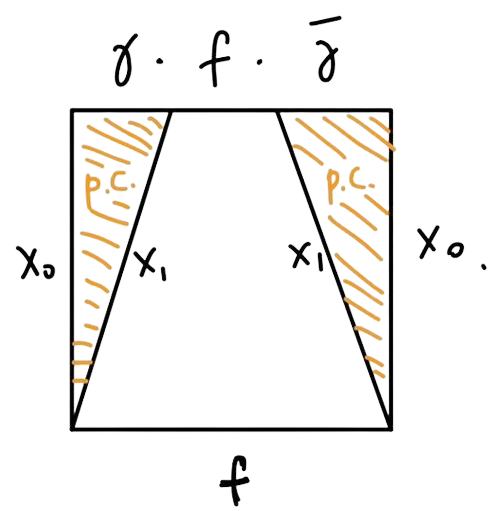
\includegraphics[scale = 0.3]{Image 1}
\end{center}

Thus $\Psi([\gamma\cdot f\cdot\overline{\gamma})=[f]$. \\~\\

Now suppose that $\Psi([f])=\Psi([g])$. Then this implies that $f\simeq g$ are free homotopic where $f$ and $g$ have basepoint $x_0$. Let $H:I\times I\to X$ be the homotopy. Let $h:I\to X$ be defined as $h(t)=H(0,t)$. Then we have 
\begin{gather*}
h(0)=H(0,0)=f(0)=x_0\\
h(1)=H(0,1)=g(0)=x_0
\end{gather*}
so that $h$ is a loop. By lemma 1.19, we have that $(H_0)_\ast=\beta_h\circ(H_1)_\ast$ if and only if $f_\ast=\beta_h\circ g_\ast$. Plugging in the generator $\omega_1$ of $\pi_1(S^1,1)\cong\Z$, we have that 
\begin{align*}
f_\ast(\omega_1)&=(\beta_h\circ g_\ast)(\omega_1)\\
f\circ\omega_1&=\beta_h(g\circ\omega_1)
\end{align*}
But $f\simeq f\circ\omega_1$ and $\overline{h}\cdot g\cdot h\simeq\beta_h(g\circ\omega_1)$ and so we have that $[f]=[\overline{h}]\cdot[g]\cdot[h]$. \\~\\

Suppose that $[f]=[\overline{\gamma}\cdot g\cdot\gamma]$ for some $\gamma:I\to X$ a loop so that $f,g,\gamma$ are loops based at $x_0$. Applying $\Psi$, we have that $\Psi([f])=\Psi([\overline{\gamma}\cdot g\cdot\gamma])$. Consider $\Psi([g])\in[S^1,X]$. It is clear that $g\in\Psi([g])$. Moreover, we must have $g\simeq\overline{\gamma}\cdot g\cdot\gamma$ by the same homotopy given above (replace $f$ with $g$). Thus we have that $f$ is free homotopic to $g$. 
\end{proof}
\end{ex}

\begin{ex}{}{} Define $f:S^1\times I\to S^1\times I$ by $f(\theta,s)=(\theta+2\pi s,s)$ so $f$ restricts to the identity on the two boundary circles $S^1\times I$. Show that $f$ is homotopic to the identity by a homotopy $f_t$ that is stationary on one of the boundary circles, but not by any homotopy $f_t$ that is stationary on both boundary circles. \tcbline
\begin{proof}
Define $H:(S^1\times I)\times I\to S^1\times I$ by $$(\theta,s,t)\mapsto(\theta+2\pi s(1-t),s)$$ Clearly $H$ is continuous. Moreover, 
\begin{align*}
H(\theta,s,0)&=f(\theta,s)\\
H(\theta,s,1)&=\text{id}(\theta,s)\\
H(\theta,0,t)&=(\theta,0)
\end{align*}
Thus we have that $$f\overset{S^1\times\{0\}}{\simeq}\text{id}$$ Now suppose that $H$ is a homotopy from $\text{id}$ to $f$ that fixes $S^1\times\{0\}$ and $S^1\times\{1\}$. Let $\gamma:I\to S^1\times I$ be a path defined as $\gamma(s)=\theta_0+s$ for some fixed $\theta_0$. Then the conditions on $H$ implies that 
\begin{align*}
H(\gamma(s),0)&=\gamma(s)\\
H(\gamma(s),1)&=(f\circ\gamma)(s)
\end{align*}
so that we have a homotopy $\gamma\simeq f\circ\gamma$. \\~\\

Consider the projection $p:S^1\times I\to S^1$. Then we have that 
\begin{align*}
\gamma&\simeq f\circ\gamma\\
p\circ\gamma&\simeq p\circ f\circ\gamma\\
e&\simeq\omega_1
\end{align*}
But $\omega_1$ is a generator of $\pi_1(S^1)$ hence this is a contradiction. 
\end{proof}
\end{ex}

\begin{ex}{}{} Does the Borsak-Ulam theorem hold for the torus? In other words, for every map $f:S^1\times S^1\to\R^2$, must there exist $(x,y)\in S^1\times S^1$ such that $f(x,y)=f(-x,-y)$? \tcbline
\begin{proof}
The Borsak-Ulam theorem fails on the torus. Consider the map $f:S^1\times S^1\subset\R^3\to\R^2$ that forgers the $z$ coordinate of the torus. It is clear that for two points to have the same image under $f$, it must have the same $y$ value in $S^1\times S^1$ (Think of the first circle in $S^1\times S^1$ having the $y$-axis passing  through and the second circle having the $z$-axis passing through). Assume that the theorem holds. Then $f(x,y)=f(-x,-y)$ together with $y=-y$ implies that $y=0$ in $\R^3$ coordinates. But not point in the torus has $\R^3$ coordinate $y=0$, which is a contradiction. 
\end{proof}
\end{ex}

\begin{ex}{}{} Let $A_1,A_2,A_3$ be compact sets in $\R^3$. Use the Borsa-Ulam theorem to show that there is one plane $P\subset\R^3$ that simultaneously divides each $A_i$ into two pieces of equal measure. \tcbline
\begin{proof}
Consider $S^2\subset\R^3$. Let $v$ be a vector in $S^2$ and consider its span which I also denote by $v$. For any scalar $p$, there is a normal plane of $v$ that passes through $pv$. In particular, there is a continuous collection of planes that slices through $A_i$ for $i=1,2,3$. Define a measure of volume in $\R^3$. Such a measure must be continuous so that the intermediate value theorem implies that there exists one such $p_i$ for which the normal plane at $p_iv$ slices $A_i$ in half by volume. \\~\\

This is because as $p$ increases in $\R$, $$\text{Vol}\left(A\cap\text{lower of half of }\R^3\text{ bounded by the normal plane}\right)$$ increases and eventually attains full volume (full volume is finite since $A_i$ is compact) so that we can apply IVT. \\~\\

Doing this for every vector $v$ in $\R^3$, we obtain a function $f:S^2\to\R^2$ defined by $f(v)=(p_1-p_3,p_2-p_3)$. By Borsak-Ulam theorem, there exists $v\in S^2$ such that $f(v)=f(-v)$ (Showing continuity of $f$ is hard!). In other words, we have that $(p_1-p_3,p_2-p_3)=(p_3-p_1,p_3-p_2)$. This implies that $p_1=p_2=p_3$. But this means that the hyperplane at $p_1v=p_2v=p_3v$ cuts through all $A_1,A_2,A_3$ and thus we conclude. 
\end{proof}
\end{ex}

\pagebreak

\section{Homology}
\subsection{Simplicial and Singular Homology}
\begin{ex}{}{} What familiar space is the quotient $\Delta$-complex of a $2$-simplex $[v_0,v_1,v_2]$ obtained by identifying the edges $[v_0,v_1]$ and $[v_1,v_2]$, preserving the order of vertices? \tcbline
\begin{proof}
By cutting through a straight line from $v_1$ down to the face $[v_0,v_2]$ perpendicularly, we can glue it back together according to the identification $[v_0,v_1]\sim[v_1,v_2]$ to obtain the following. 

\begin{center}
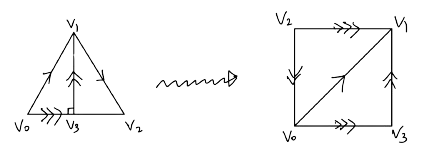
\includegraphics[scale = 0.8]{Image 2}
\end{center}

It is then clear that this is a Möbius strip. 
\end{proof}
\end{ex}

\begin{ex}{}{} Show that the $\Delta$-complex obtained from $\Delta^3$ by performing the edge identifications $[v_0,v_1]\sim[v_1,v_3]$ and $[v_0,v_2]\sim[v_2,v_3]$ deformation retracts onto a Klein bottle. Find other pairs of identifications of edges that produce $\Delta$-complexes deformation retracting onto a torus, a $2$-sphere and $\R\Prj^2$. \tcbline
\begin{proof}
Notice that the face $[v_0,v_1,v_3]$ can be deformation retracted onto the union of $[v_0,v_1]$ and $[v_1,v_3]$ so that $\Delta^3$ is now a square with two faces $[v_0,v_2,v_1]$ and $[v_2,v_1,v_3]$ as follows 

\begin{center}
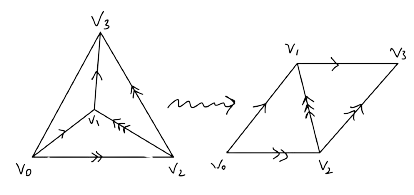
\includegraphics[scale = 0.8]{Image 4}
\end{center}

Then by cutting along the $1$-simplex $[v_1,v_2]$ an gluing it back up along the identified edges $[v_0,v_2]$ and $[v_2,v_3]$, we obtain the following 

\begin{center}
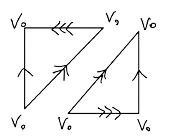
\includegraphics[scale = 0.8]{Image 5}
\end{center}

It is then clear that this is precisely the $\Delta$-complex structure of the Klein bottle. \\~\\

For the torus, the identification is $[v_0,v_1]\sim[v_2,v_3]$ and $[v_0,v_2]\sim[v_1,v_3]$ and then deformation retracting the same face $[v_0,v_1,v_3]$ onto the union of $[v_0,v_1]$ and $[v_1,v_3]$. No edges should be identified to form the $2$-sphere since $\Delta^3$ is already homeomorphic to the sphere. Finally, $\R\Prj^2$ is obtained by identifying $[v_0,v_2]\sim[v_3,v_1]$ and $[v_0,v_1]\sim[v_3,v_3]$ in the order of the vertices mentioned. 
\end{proof}
\end{ex}

\begin{ex}{}{} Construct a $\Delta$-complex structure on $\R\Prj^n$ as a quotient of a $\Delta$-complex structure on $S^n$ having vertices the two vectors of length $1$ along each coordinate axis in $\R^{n+1}$ \tcbline
\begin{proof}
Write the unit vectors of $\R^{n+1}$ by $e_0,\dots,e_n$ and its negatives by $-e_0,\dots,-e_n$. A $\Delta$-complex structure of $S^n$ can be obtained as follows. The $n$-simplexes for $0\leq k\leq n$ are the simplexes of the form $[\pm e_0,\dots,\pm\hat{e}_i,\dots,\pm e_n]$ where the hat means that $\hat{e}_i$ is omitted so that it indeed denotes an $n$-simplex. The $k$-simplexes are then precisely the boundaries of the $(k+1)$-simplexes for $0\leq k\leq n-1$ and the $0$-simplexes are then precisely the points $\pm e_0,\dots,\pm e_n$. For $[(-1)^{a_0}e_0,\dots,(-1)^{a_n}e_n]$ an $n$-simplex, identify it with $$[(-1)^{a_0+1}e_0,\dots,(-1)^{a_n+1}e_n]$$ This identification on $S^n$ gives precisely $\R\Prj^2$ because for any point $v$ on the $n$-simplex, it is identified with $-v$. 
\end{proof}
\end{ex}

\begin{ex}{}{} Compute the simplicial homology groups of the triangular parachute obtained from $\Delta^2$ by identifying its three vertices to a single point. \tcbline
\begin{proof}
The triangular parachute has a $\Delta$ complex structure with one $0$-simplex $p$, three $1$-simplexes $a,b,c$ with boundary the only simplex, and $2$-simplex with boundary $b-c+a$ given by the following picture: 

\begin{center}
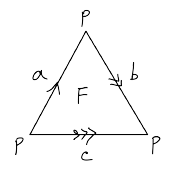
\includegraphics[scale = 0.8]{Image 3}
\end{center}

This means that we have the following chain complex: \\~\\
\adjustbox{scale=1.0,center}{\begin{tikzcd}
	0 & \Z & {\Z^3} & \Z & 0
	\arrow[from=1-1, to=1-2]
	\arrow["{d_2}", from=1-2, to=1-3]
	\arrow["{d_1}", from=1-3, to=1-4]
	\arrow[from=1-4, to=1-5]
\end{tikzcd}}\\~\\
The matrix of $d_1$ and $d_2$ are given by $$d_1=0\;\;\;\;\text{ and }\;\;\;\; d_2=\begin{pmatrix}
1\\1\\-1
\end{pmatrix}$$ respectively. Then the Smith normal form of $d_2$ is just $\begin{pmatrix}
1\\0\\0
\end{pmatrix}$ and thus the homology groups are given as $$H_n(X)=\begin{cases}
\Z & \text{ if } n=0\\
\Z^2 & \text{ if } n=1\\
0 & \text{ otherwise }
\end{cases}$$
\end{proof}
\end{ex}

\begin{ex}{}{} Compute the simplicial homology groups of the Klein bottle using the $\Delta$-complex structure described at the beginning of this section. \tcbline
\begin{proof}
The $\Delta$-complex structure of the Klein bottle described consists of one $0$-simplex $v$, three $1$-simplexes $a,b,c$ and two $2$-simplexes $U$ and $L$. This means that this gives its simplicial chain complex as \\~\\
\adjustbox{scale=1.0,center}{\begin{tikzcd}
	0 & \Z^2 & {\Z^3} & \Z & 0
	\arrow[from=1-1, to=1-2]
	\arrow["{d_2}", from=1-2, to=1-3]
	\arrow["{d_1}", from=1-3, to=1-4]
	\arrow[from=1-4, to=1-5]
\end{tikzcd}}\\~\\
Since there is only one $0$-simplex, every $1$-simplex has boundary $v-v=0$ and so $d_1$ is the zero map. From the $\Delta$-complex structure, the boundary of $U$ can be seen to be oriented by $a,b$ and $c$. So we have that $d_2(U)=b-c+a$. Similarly, we have that $d_2(L)=a-b+c$. Thus the matrix of the map $d_2:\Z^2\to\Z^3$ can be written as $$\begin{pmatrix}
1 & 1\\
1 & -1\\
1 & -1
\end{pmatrix}\overset{\text{SNF}}{\longrightarrow}\begin{pmatrix}
1 & 0\\
0 & 2\\
0 & 0
\end{pmatrix}$$ where SNF mean the Smith normal form. It is easy to see that $\ker(d_2)=0$ and $\im(d_2)\cong \Z\oplus 2\Z$. Thus we have that $$H_n(K)=\begin{cases}
\Z & \text{ if } n=0\\
\Z/2\Z & \text{ if } n=1\\
0 & \text{ otherwise }
\end{cases}$$
\end{proof}
\end{ex}

\begin{ex}{}{} Compute the simplicial homology groups of the $\Delta$-complex obtained from $n+1$ $2$-simplices $\Delta_0^2,\dots,\Delta_n^2$ by identifying all three edges of $\Delta_0^2$ to a single edge, and for $i>0$ identifying the edges $[v_0,v_1]$ and $[v_1,v_2]$ of $\Delta_i^2$ to a single edge and the edge $[v_0,v_2]$ to the edge $[v_0,v_1]$ of $\Delta_{i-1}^2$. 
\end{ex}

\begin{ex}{}{} Find a way of identifying pairs of faces of $\Delta^3$ to produce a $\Delta$-complex structure on $S^3$ having a single $3$-simplex, and compute the simplicial homology groups of this $\Delta$-complex. \tcbline
\begin{proof}
Identify the faces of $\Delta^3$ via $[v_0,v_1,v_2]\sim[v_0,v_1,v_3]$ and $[v_0,v_2,v_3]\sim[v_1,v_2,v_3]$. The first identification can be visualized as follows: hold the two points $v_2$ and $v_3$ of $\Delta^3$ and move it along a circular arc, thinking of $[v_2,v_3]$ as the diameter. 

\begin{center}
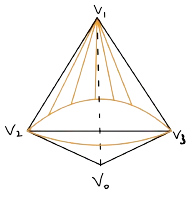
\includegraphics[scale = 0.8]{Image 6}
\end{center}

Gluing the faces, together, we obtain the following: 

\begin{center}
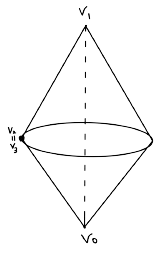
\includegraphics[scale = 0.8]{Image 7}
\end{center}

This is homeomorphic to $D^3$ by thinking of $v_1$ and $v_0$ as the north and south poles respectively, and then inflating it. Now it is known that $$S^3\cong\frac{D^3}{\sim}$$ where $v\sim -v$ for $v\in\partial D$. Then the identification of $[v_0,v_2,v_3]\sim[v_1,v_2,v_3]$ in $\Delta^3$ is precisely taking $D^3$ and then defining the same equivalence relation on $\partial D^3\cong S^2$. Thus we know have $\Delta^3$ being a $\Delta$-complex structure on $S^3$. 

To compute the homology groups, notice that there are now two $0$-simplexes $[v_0]\sim[v_1]$ and $[v_2]\sim[v_3]$. There are three $1$-simplexes $[v_2,v_2=v_3]$, $[v_1,v_2]\sim[v_0,v_2]\sim[v_1,v_3]\sim[v_0,v_3]$ and $[v_0,v_0=v_1]$. There are two $2$-simplexes $[v_0,v_2,v_3]\sim[v_1,v_2,v_3]$ and $[v_0,v_1,v_2]\sim[v_0,v_1,v_3]$ and one $3$-simplex $[v_0,v_1,v_2,v_3]$. The simplicial chain complex is thus \\~\\
\adjustbox{scale=0.8,center}{\begin{tikzcd}
	0 & {\Z[v_0,v_1,v_2,v_3]} & {\Z[v_0,v_1,v_2]\oplus\Z[v_0,v_2,v_3]} & {\Z[v_0,v_1]\oplus\Z[v_1,v_2]\oplus\Z[v_2,v_3]} & {\Z[v_0]\oplus\Z[v_2]} & 0
	\arrow[from=1-1, to=1-2]
	\arrow[from=1-2, to=1-3]
	\arrow[from=1-3, to=1-4]
	\arrow[from=1-4, to=1-5]
	\arrow[from=1-5, to=1-6]
\end{tikzcd}}\\~\\
The boundary maps can be understood as follows. The first boundary map can be computed as \begin{align*}
d_1([v_0,v_1])&=[v_1]-[v_0]=0\\
d_1([v_1,v_2])&=[v_2]-[v_1]=[v_2]-[v_0]\\
d_1([v_2,v_3])&=[v_3]-[v_2]=0
\end{align*}
Then the second boundary map: 
\begin{align*}
d_2([v_0,v_1,v_2])&=[v_1,v_2]-[v_0,v_2]+[v_0,v_1]=[v_1,v_2]-[v_1,v_2]+[v_0,v_1]=[v_0,v_1]\\
d_2([v_0,v_2,v_3])&=[v_2,v_3]-[v_0,v_3]+[v_0,v_2]=[v_2,v_3]
\end{align*}
And the last one: $$d_3([v_0,v_1,v_2,v_3])=[v_1,v_2,v_3]-[v_0,v_2,v_3]+[v_0,v_1,v_3]-[v_0,v_1,v_2]=0$$
We can write them in to a matrix so that 
\begin{gather*}
d_1=\begin{pmatrix}
0 & -1 & 0\\
0 & 1 & 0
\end{pmatrix}\;\;\;\;\overset{\text{SNF}}{\longrightarrow}\;\;\;\;\begin{pmatrix}
1 & 0 & 0\\
0 & 0 & 0
\end{pmatrix}\\
d_2=\begin{pmatrix}
1 & 0\\
0 & 0\\
0 & 1
\end{pmatrix}\;\;\;\;\overset{\text{SNF}}{\longrightarrow}\;\;\;\;\begin{pmatrix}
1 & 0\\
0 & 1\\
0 & 0
\end{pmatrix}\\
d_3=\begin{pmatrix}
0\\
0
\end{pmatrix}
\end{gather*}
Then the homology groups can be read off as $$H_n(S^3)=\begin{cases}
\Z & \text{ if } n=0,3\\
0 & \text{ otherwise }
\end{cases}$$
which one can check is precisely the singular homology of $S^3$. 
\end{proof}
\end{ex}

\begin{ex}{}{} Compute the homology groups of the $\Delta$-complex $X$ obtained from $\Delta^n$ by identifying all faces of the same dimension. Thus $X$ has a single $k$-simplex for each $k\leq n$. \tcbline
\begin{proof}
It is clear that the simplicial chain complex of $X$ is just one copy of $\Z$ on dimensions $0,1,\dots,n$. We have to understand the boundary maps. For a $k$-simplex $[v_0,\dots,v_k]$, we have the formula $$d_k([v_0,\dots,v_k])=\sum_{i=0}^k(-1)^i\sigma[v_0,\dots,\hat{v}_i,\dots,v_k]$$ In $X$, there is only one $(k-1)$-simplex so the formula becomes $$d_k([v_0,\dots,v_k])=\begin{cases}
0 & \text{ if } 0\leq k\leq n \text{ is odd}\\
[v_0,\dots,\hat{v}_i,\dots,v_k] & \text{ if } 0\leq k\leq n \text{ is even}
\end{cases}$$
This means that $d_k$ is either the identity or the zero map. When $0<k<n$ is even, we have that $$H_k(X)=\frac{\ker(d_k)}{\im(d_{k+1})}=\frac{\ker(\text{id})}{\im(0)}\cong 0$$ When $0<k<n$ is odd, we have that $$H_k(X)=\frac{\ker(d_k)}{\im(d_{k+1})}=\frac{\ker(0)}{\im(\text{id})}\cong 0$$ When $k=0$, we have $H_0(X)=\Z$. When $k=n$ and $n$ is odd, we have that $H_n(X)=\Z$. When $k=n$ and $n$ is even, we have that $H_n(X)=0$. 
\end{proof}
\end{ex}



\end{document}
